\documentclass[a4paper,11pt]{article}

\usepackage[utf8]{inputenc}

\usepackage{graphicx}
\usepackage{caption}
\usepackage{subcaption}

\usepackage{pgfplots}
\usepackage{float}
\usepackage{hyperref}
\usepackage{soul}
\hypersetup{
    colorlinks=true, % Enable colored links
    linkcolor=black, % Color for internal links
    urlcolor=black,  % Color for external links
    citecolor=black, % Color for citation links
    pdfborder={0 0 0}, % Remove border around links
}
\newcommand{\underlinehref}[2]{%
    \href{#1}{\ul{#2}}%
}
\pgfplotsset{compat=1.18}


\usepackage{minted}

\begin{document}

    \title{
        \textbf{Wrap around Queues in C}
    }
    \author{Péter Herczku}
    \date{Fall 2024}

    \maketitle

    \section*{Introduction}

    The task is to implement the queue structure using the wrap around algorithm and benchmark its operations.

    I completed the assignment using the C programming language.

    \section*{Using an array}

    In the previous assignment, the queue data structure was implemented using a linked list, but we needed to allocate new memory every time a new node was added which led to extra overhead.
    We can utilize an array instead, where we don't need to deal with this overhead, however we still need to extend the array when we hit its limitations.

    \section*{Wrap around}

    This algorithm stores the queue in an array and holds the array's size and two indexes: one that points to the first element that should be dequeued and another pointing to the next free spot in the array.

    \begin{minted}{c}
typedef struct queue {
    int firstIndex;
    int lastIndex;
    int* array;
    int size;
} queue;
    \end{minted}

    \subsection*{Enqueue}

    The idea behind this algorithm is that when an element is enqueued, it is placed in the array at the position {\tt lastIndex}, and then we increment {\tt lastIndex}.
    But what happens when we increment lastIndex, and it's outside our array?
    In C we can do that, but it leads to unpredictable behavior.
    Instead, we can go back to the beginning of the array, and if the spot is available we can write there.
    But how can we know that it's available?
    After each enqueue operation we check if {\tt lastIndex} equals {\tt firstIndex}: if it's true then we filled up the array completely, and we need to extend it.
    Therefore, we make sure after each call of the method that it's safe to {\tt enqueue} next time.

    Let's implement our enqueue function:

    \begin{minted}{c}
void enqueue(queue* q, int value) {
    q->array[q->lastIndex] = value;
    q->lastIndex = (q->lastIndex + 1) % q->size;
    if(q->firstIndex == q->lastIndex) {
        int* newArray = (int*) malloc(sizeof(int)*q->size*2);
        int k = 0;
        for(int i = q->lastIndex; i < q->size; i++) {
            newArray[k] = q->array[i];
            k++;
        }
        for(int i = 0; i < q->lastIndex; i++) {
            newArray[k] = q->array[i];
            k++;
        }
        q->firstIndex = 0;
        q->lastIndex = k;
        int* arr = q->array;
        q->array = newArray;
        free(arr);
        q->size = q->size * 2;
    }
}
    \end{minted}

    After incrementing our {\tt lastIndex} value we need to take {\tt mod size}, so it can go back to the beginning of the array: this is why this algorithm is called wrap around.
    When our array becomes full, we copy the entire array into a new one, but we need to keep the right order of elements.
    Therefore, we first copy the elements from firstIndex until the end of the array, and then the rest.
    After that we set up our pointers and the new array accordingly.

    \subsection*{Dequeue}

    In our {\tt dequeue} function, we retrieve the value at position {\tt firstIndex}, and we store this value in a temporary variable, because we need to increment our {\tt firstIndex} pointer as well.
    In order to utilize the wrap around method, we need to take {\tt mod size} after incrementing the pointer.
    After doing all this, we can finally return the value we retrieved.

    \begin{minted}{c}
int dequeue(queue* q) {
    if(q->firstIndex == q->lastIndex) return -1;
    int val = q->array[q->firstIndex];
    q->firstIndex = (q->firstIndex + 1) % q->size;
    return val;
}
    \end{minted}

    We also need to consider an edge case, when the queue is empty: in this case we return an unusual value, in this case $-1$.

    \section*{Benchmarking}

    Now that we have implemented the data structure, we can finally do some benchmarking.
    In the benchmark, I analyzed the time complexity for the {\tt enqueue} and {\tt dequeue} functions by calling them after each other.
    Let's take a look at our results:

    \begin{figure}[H]
        \centering
        \begin{subfigure}[b]{.5\textwidth}
            \centering
            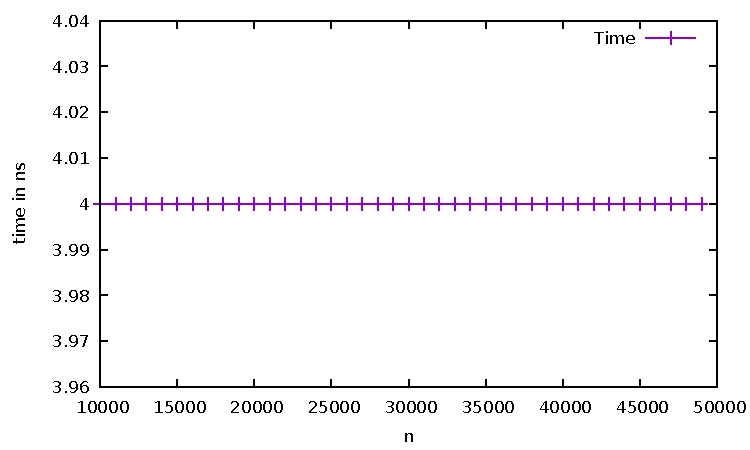
\includegraphics[width=\textwidth]{./src/data} % Adjust width or height as needed
        \end{subfigure}
        \caption{Graph of wrap around}
        \label{fig:graph_1}
    \end{figure}

    The graph shows a constant relationship, which means that the time complexity for both {\tt enqueue} and {\tt dequeue} is $O(1)$, which is highly efficient.
    However, in the benchmark we didn't need to extend our array because we called the {\tt dequeue} function first, but we had learned that if we keep doubling the size of the array, the time complexity will still be $O(1)$.

    \section*{Array resizing}

    We need to consider the edge case, when the array becomes very large, but all elements have been already dequeued.
    The implementation is a bit more advanced, and will not be discussed in detail in this report, but it's worth mentioning it.

    We can add an extra check for the {\tt dequeue} function that will shrink the array when the actual size is {\tt size/4}.
    In order to do this, we can add an extra property to our structure that holds the length of the queue.

    \begin{minted}{c}
typedef struct queue {
    ...
    int length;
} queue;
    \end{minted}

    In the {\tt dequeue} function, we need to resize the array to {\tt size/2}, when the {\tt length} reaches the critical size: {\tt size/4}.

    \section*{Array vs Linked list}

    After improving our implementation in the last assignment we managed to get $O(1)$ time complexity.
    However, the actual runtime seems is slightly better for the wrap around implementation.
    This could be due to the fact we do not need to allocate new memory at each {\tt enqueue} operation.

    \section*{GitHub}
    I have uploaded the full project to \underlinehref{https://github.com/peterherczku/ID1021/tree/main/assignment-6-D}{my github repository}, where we can find the code used to make this report.

\end{document}
